\documentclass[10pt, a4paper, reprint, amsmath,amssymb, aps]{revtex4-2}

\usepackage{graphicx}
\usepackage{dcolumn}
\usepackage{bm}
\usepackage[top=0.5in, bottom=0.3in, left=0.1in, right=0.1in]{geometry}

\usepackage{lipsum}

\usepackage{setspace}

\usepackage{fancyhdr}
\setlength{\parindent}{0in}

% Page Formatting
\pagenumbering{arabic} %\pagenumbering{gobble}
\onehalfspacing %doublespacing
\pagestyle{fancy}
%\usepackage{pdfpages}

% Heading Formatting
\headheight 32pt

% Link Formatting
\usepackage{hyperref}
\hypersetup{
	colorlinks,
	allcolors=black
	%citecolor=black,
	%filecolor=black,
	%linkcolor=black,
	%urlcolor=black
}

\usepackage{mdframed}

% Code Formatting
\usepackage{listings}
% \lstset{
%         language=Python,
% 	basicstyle=\footnotesize,
% 	%numbers=left,
% 	stepnumber=1,
% 	showstringspaces=false,
% 	tabsize=1,
% 	breaklines=true,
% 	breakatwhitespace=false
% }

\lstset
{ %Formatting for code  
        language=Python,
	basicstyle=\footnotesize\ttfamily,
	numbers=left,
	%caption={},
	%title={},
	stepnumber=1,
	showstringspaces=false,
	tabsize=1,
	breaklines=true,
	breakatwhitespace=false,
	frame=lines,
	xleftmargin=2em,
	framexleftmargin=1.5em,
	%commentstyle=\color{commentsColor}\ttfamily,
  	%stringstyle=\color{stringColor}\ttfamily,
	%keywordstyle=\color{keywordsColor}\bfseries,
}

% Figures & Drawings
%\usepackage{graphicx, caption}
%\usepackage{animate}
\usepackage{tikz}
\usepackage{float}
\usepackage{pict2e}
\usepackage{subcaption}

% Physics
\usepackage{physics}

% Mathematics
\usepackage{amsmath}
\usepackage{amssymb}
\usepackage{amsthm}
\usepackage{mathtools}
\usepackage{mathrsfs}
\usepackage{upgreek} % More Greek letters

% I don't really know what this is but I don't want to break shit
\usepackage{aliascnt}
\newaliascnt{eqfloat}{equation}
\newfloat{eqfloat}{h}{eqflts}
\floatname{eqfloat}{Equation}
\newcommand*{\ORGeqfloat}{}
\let\ORGeqfloat\eqfloat
\def\eqfloat{%
	\let\ORIGINALcaption\caption
	\def\caption{%
		\addtocounter{equation}{-1}%
		\ORIGINALcaption
	}%
	\ORGeqfloat
}
%}

% Bibliography (Citations) Formatting

%\usepackage{cite}
%\usepackage{caption}

%\usepackage[backend=bibtex,style=verbose-trad2]{biblatex}
%works really really well, but no MLA format
%\bibliographystyle{apsrev4-1}
%\usepackage{biblatex}
%\usepackage[backend=biber]{biblatex}
%\usepackage[backend=biber,style=mla]{biblatex} %Doesn't print all sources for some reason

\usepackage{pgfplots}

\input{preamble/tikz}
\input{preamble/macros}

% ========================================= %
% Change for each document [!!!]
\newcommand\course{PHY365}	% Course Code [!!!]
\newcommand\doctitle{Final Formula Sheet} % Report Title [!!!]
\newcommand\firstauthorname{Aditya K. Rao 1008307761}
%\newcommand\firstauthorname{\textbf{Name:}}
\newcommand\taname{D.F.V. James} % TA Name [!!!]
\newcommand{\location}{\texttt{April 25, 2024}} % Location [!!!]
% ========================================= %
 
%\pagenumbering{gobble}
\usepackage{listings}

\renewcommand\lstlistingname{Code Reference}
\renewcommand\lstlistlistingname{Code Reference}
\usepackage{tikz}
\usetikzlibrary{patterns}

\setlength{\belowdisplayskip}{0pt} \setlength{\belowdisplayshortskip}{0pt}
\setlength{\abovedisplayskip}{0pt} \setlength{\abovedisplayshortskip}{0pt}

\begin{document}
\lhead{\firstauthorname\vspace{0.1cm}}
\chead{\textbf{\course} \\ \doctitle}
\rhead{\textbf{Prof:} \taname \\ \textbf{Date:} \location}

\section{Pauli Matrices \& Gates}
\vspace{-1cm}
    \begin{gather*}
        \hat{I} = \hat{\sigma_0} = \begin{bmatrix} 1 & 0 \\ 0 & 1\end{bmatrix} \ 
        \hat{X} = \hat{\sigma_1} = \begin{bmatrix} 0 & 1 \\ 1 & 0\end{bmatrix} \
        \hat{Y} = \hat{\sigma_2} = \begin{bmatrix} 0 & -i \\ i & 0\end{bmatrix} \\ 
         \hat{Z} = \hat{\sigma_3} = \begin{bmatrix} 1 & 0 \\ 0 & -1\end{bmatrix} \ \hat{H} = \frac{1}{\sqrt{2}}(\hat{X}+\hat{Z}) = \frac{1}{\sqrt{2}}\begin{bmatrix} 1 & 1 \\ 1 & -1\end{bmatrix}
    \end{gather*}
    \begin{gather*}
        \hat{X}\hat{Y} = i\hat{Z} = -\hat{Y}\hat{X} \ \
        \hat{Z}\hat{X} = i\hat{Y} = -\hat{X}\hat{Z} \\
        \hat{Y}\hat{Z} = i\hat{X} = -\hat{Z}\hat{Y} \ \
        \hat{X}\hat{X} = \hat{Y}\hat{Y} = \hat{Z}\hat{Z} = \hat{I} \\
        \hat{\sigma_i}\hat{\sigma_j} = \hat{I}\delta_{ij}+i\sum\limits_{k=1}^{3}\epsilon_{ijk}\hat{\sigma_k}
    \end{gather*}
    Where $\delta$ is the \textit{Kr{\"o}necker delta}, and $\epsilon$ is the Levi-Civita symbol.
    \begin{equation*} \label{eqn:pauli-euler}
        \exp{i\theta \mathbf{n}\cdot\hat{\sigma}} = \cos\theta\hat{I}+i\sin\theta\mathbf{n}\cdot\hat{\sigma}
    \end{equation*}
    \begin{gather*}
        \texttt{MEASUREMENT} = \ket{u}\bra{u}, \ket{v}\bra{v} \ , \ \ket{0}\bra{0}X = X\ket{1}\bra{1}
        \\
        \texttt{CNOT} = \ket{0}\bra{0}\otimes\hat{I} + \ket{1}\bra{1}\otimes\hat{X} \\
        \hat{U} = \begin{bmatrix}a & b \\ -b^* & a^*\end{bmatrix}, \  \hat{U}\hat{U}^\dagger =  \hat{I}
    \end{gather*}
    \begin{gather*}
        \texttt{SWAP} = 
        \begin{bmatrix}
            1 & 0 & 0 & 0 \\
            0 & 0 & 1 & 0 \\
            0 & 1 & 0 & 0 \\
            0 & 0 & 0 & 1
        \end{bmatrix} \ 
        \sqrt{\texttt{SWAP}} = 
        \begin{bmatrix}
            1 & 0 & 0 & 0 \\
            0 & (1+i)/2 & (1-i)/2 & 0 \\
            0 & (1-i)/2 & (1+i)/2 & 0 \\
            0 & 0 & 0 & 1
        \end{bmatrix}
    \end{gather*}
\section{Miscellaneous}
    \vspace{6.2cm}

\section{Bell's Inequalities \& Bell States}
    \begin{align*}
        \beta_0 = \frac{1}{\sqrt{2}} (\ket{00} + \ket{11}) \ & \ \beta_1 = \frac{1}{\sqrt{2}} (\ket{00} - \ket{11})\\
        \beta_2 = \frac{1}{\sqrt{2}} (\ket{01} - \ket{10}) \ & \ 
        \beta_3 = \frac{1}{\sqrt{2}} (\ket{01} + \ket{10})
    \end{align*}
    \begin{center}
        \begin{quantikz}
        \lstick{$\ket{x}$} & \gate{H}&\ctrl{1} & \rstick[2]{$\beta_{xy} = \frac{\ket{0}\ket{y} + (-1)^x\ket{1}\ket{\overline{y}}}{\sqrt{2}}, \overline{y} \ \text{is negation of y}$} \\
        \lstick{$\ket{y}$} & & \targ{} &
        \end{quantikz}
    \end{center}

\section{Concurrence and Schmidt Decomposition}
    \textbf{Local unitaries do not effect concurrence}.
    \begin{minipage}{\linewidth}
    \begin{minipage}{0.49\linewidth}
        \begin{gather*} 
            \ket{\varphi} = \alpha\ket{00} + \beta\ket{01} + \gamma\ket{10} + \delta\ket{11} \\
            = \lambda_0\ket{u_0}\ket{v_0} + \lambda_1\ket{u_1}\ket{v_1}
        \end{gather*}
    \end{minipage}
    \begin{minipage}{0.49\linewidth}
        \begin{gather*}
            \chi = \begin{bmatrix}
                \alpha & \beta \\ \gamma & \delta
            \end{bmatrix}
        \end{gather*}
        Positive value of $\chi\chi^\dagger$ will be schmidt numbers.
    \end{minipage}
    \end{minipage}
        \begin{gather*}
            C = 2|\alpha\delta - \beta\gamma| = 2\lambda_0\lambda_1 = \begin{cases}0 & \text{Not at all entangled}\\1 & \text{Completely entangled}\end{cases} \\
            \lambda_0^2 + \lambda_1^2 = 1 \ \ \lambda^2 = \frac{1\pm\sqrt{1-C^2}}{2}
        \end{gather*}
        \begin{theorem} \textbf{The Fundamental Theorem of Entanglement}
            \begin{align*}
                (I\otimes U)\ket{\beta_2} =& -\frac{1}{\sqrt{2}} (\ket{0}\otimes(b\ket{0}+a^*\ket{1})
                -\ket{1}\otimes(a\ket{0}-b^*\ket{1})) \\
                =& -(U^\dagger\otimes I )\ket{\beta_2} 
                \therefore (U\otimes U)\ket{\beta_2} = -\ket{\beta_2}
            \end{align*}

            A unitary applied to $\Q_0$ in a maximally entangled (in singlet basis) pair is equivalent to applying a related unitary to $\Q_1$ of the pair.

        \end{theorem}

\section{Useful Circuit Identities}
    \begin{center}
        \textbf{Griffiths-Niu Theorem}\\
        \begin{quantikz}
            & \meter{} & \ctrl[vertical wire=c]{1}\setwiretype{c} \\
            & &\gate{U}\wire[u][1]{c}
        \end{quantikz}
        $\equiv$
         \begin{quantikz}
            & \ctrl{1} & \meter{} & \setwiretype{c} \\
            & \gate{U} & &
        \end{quantikz}
    \end{center}
    \begin{center}
        \begin{quantikz}
            & \ctrl{1} & & \ctrl{1} & & \\
            & \targ{} & \ctrl{1} & \targ{} & \ctrl{1} &\\
            & & \targ{} & & \targ{} & 
        \end{quantikz}
        $=$ 
        \begin{quantikz}
            & \ctrl{2} & \\
            & & \\
            & \targ{} & 
        \end{quantikz}
    \end{center}
    \begin{center}
        \textbf{Symmetry of $\hat{Z}$} \\
        \begin{quantikz}
            & \ctrl{1} & \\
            & \gate{Z} & 
        \end{quantikz}
        $=$ 
        \begin{quantikz}
            & \gate{Z} & \\
            & \ctrl{-1} & 
        \end{quantikz}
        $=$
        \begin{quantikz}
            & \gate{} & \\
            & \gate{} \wire[u][1]{q} & 
        \end{quantikz}
    \end{center}
    \begin{center}
        \textbf{\texttt{SWAP} Gate} \\
        \begin{quantikz}
            & \ctrl{1} & \targ{} & \ctrl{1} & \\
            & \targ{} & \ctrl{-1} & \targ{} &
        \end{quantikz}
        $=$ 
        \begin{quantikz}
            & \swap{1} & \\
            & \targX{} & 
        \end{quantikz}
    \end{center}

\section{Representation of Numbers \& Physical Implementation}
    For some 3 bit number $x = \{x_0, x_1, x_2\} = \sum_{n=0}^2x_n2^n$
    \begin{gather*}
        \ket{\psi(x)} = \frac{1}{2}(\ket{11} + \zeta_2\ket{10} + \zeta_1\ket{01}) + \zeta_0\ket{10}, \ \zeta_n  = 2x_n - 1 
    \end{gather*}
    \textbf{Trapped Ion Systems}\\
    \textit{Implementation of ctrl-z gate}
    \begin{center}
    \begin{minipage}{0.49\linewidth}
    \scalebox{0.6}{
    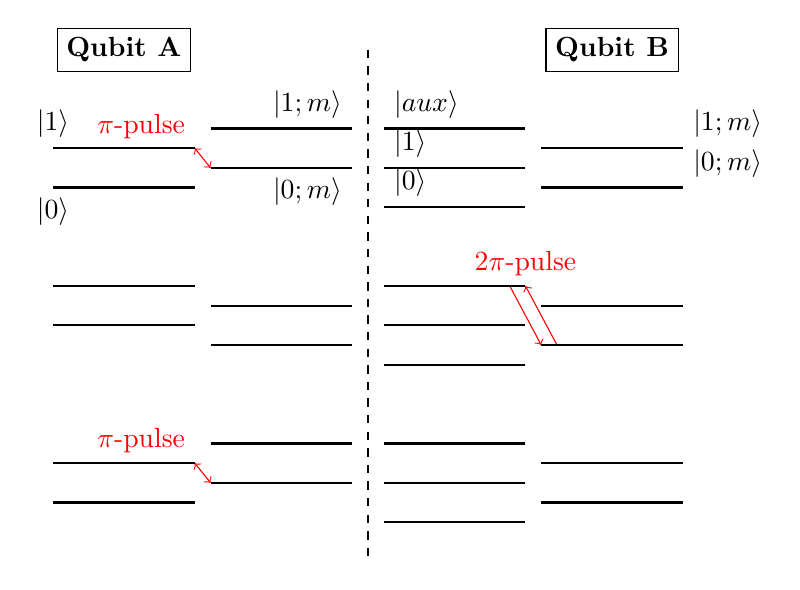
\begin{tikzpicture}
        \def\x{0.25}
        \def\va{3}
        \def\vb{1}
        \def\vc{-1}
        \draw[dashed] (0,4) -- (0,-2.5);
        
        % Pi Pulse A
        \draw[<->,red] (-2.2, \va-1*\x)node [anchor=south east] {$\pi$-pulse} -- (-2, \va-2*\x);
        % Qubit A
        \node[draw] at (-3.1,4) {\textbf{Qubit A}};
        \draw[thick] (-4,\va-1*\x)node[anchor=south]{$\ket{1}$} -- (-2.2,\va-1*\x); % 0 stationary
        \draw[thick] (-2,\va-0*\x) -- (-0.2,\va-0*\x)node[anchor=south east]{$\ket{1;m}$}; % 0 moving
        \draw[thick] (-4,\va-3*\x)node[anchor=north]{$\ket{0}$} -- (-2.2,\va-3*\x); % 1 stationary
        \draw[thick] (-2,\va-2*\x) -- (-0.2,\va-2*\x)node[anchor=north east]{$\ket{0;m}$}; % 1 moving

        % Qubit B
        \node[draw] at (3.1,4) {\textbf{Qubit B}};
        \draw[thick] (2,\va-0*\x) -- (0.2,\va-0*\x)node[anchor=south west]{$\ket{aux}$}; % aux
        \draw[thick] (4,\va-1*\x)node[anchor=south west]{$\ket{1;m}$} -- (2.2,\va-1*\x); % 0 stationary
        \draw[thick] (2,\va-2*\x) -- (0.2,\va-2*\x)node[anchor=south west]{$\ket{1}$}; % 0 moving
        \draw[thick] (4,\va-3*\x)node[anchor=south west]{$\ket{0;m}$} -- (2.2,\va-3*\x); % 1 stationary
        \draw[thick] (2,\va-4*\x) -- (0.2,\va-4*\x)node[anchor=south west]{$\ket{0}$}; % 1 moving

        % 2Pi Pulse B
        \draw[<-,red] (2,\vb-0*\x)node [above] {$2\pi$-pulse} -- (2.4,\vb-3*\x);
        \draw[->,red] (1.8,\vb-0*\x) -- (2.2,\vb-3*\x);
        % Qubit A
        \draw[thick] (-4,\vb-0*\x) -- (-2.2,\vb-0*\x); % 0 stationary
        \draw[thick] (-2,\vb-1*\x) -- (-0.2,\vb-1*\x); % 0 moving
        \draw[thick] (-4,\vb-2*\x) -- (-2.2,\vb-2*\x); % 1 stationary
        \draw[thick] (-2,\vb-3*\x) -- (-0.2,\vb-3*\x); % 1 moving

        % Qubit B
        \draw[thick] (2,\vb-0*\x) -- (0.2,\vb-0*\x); % aux
        \draw[thick] (4,\vb-1*\x) -- (2.2,\vb-1*\x); % 0 stationary
        \draw[thick] (2,\vb-2*\x) -- (0.2,\vb-2*\x); % 0 moving
        \draw[thick] (4,\vb-3*\x) -- (2.2,\vb-3*\x); % 1 stationary
        \draw[thick] (2,\vb-4*\x) -- (0.2,\vb-4*\x); % 1 moving

        % Pi Pulse A
        \draw[<->,red] (-2.2, \vc-1*\x)node [anchor=south east] {$\pi$-pulse} -- (-2, \vc-2*\x);
        % Qubit A
        \draw[thick] (-4,\vc-1*\x) -- (-2.2,\vc-1*\x); % 0 stationary
        \draw[thick] (-2,\vc-0*\x) -- (-0.2,\vc-0*\x); % 0 moving
        \draw[thick] (-4,\vc-3*\x) -- (-2.2,\vc-3*\x); % 1 stationary
        \draw[thick] (-2,\vc-2*\x) -- (-0.2,\vc-2*\x); % 1 moving

        % Qubit B
        \draw[thick] (2,\vc-0*\x) -- (0.2,\vc-0*\x); % aux
        \draw[thick] (4,\vc-1*\x) -- (2.2,\vc-1*\x); % 0 stationary
        \draw[thick] (2,\vc-2*\x) -- (0.2,\vc-2*\x); % 0 moving
        \draw[thick] (4,\vc-3*\x) -- (2.2,\vc-3*\x); % 1 stationary
        \draw[thick] (2,\vc-4*\x) -- (0.2,\vc-4*\x); % 1 moving
    \end{tikzpicture}}
    \end{minipage}
    \begin{minipage}{0.49\linewidth}
        \begin{gather*}
            \ket{00}\rightarrow\ket{00}\rightarrow\ket{00}\rightarrow\ket{00}\\
            \ket{01}\rightarrow\ket{01}\rightarrow\ket{01}\rightarrow\ket{01}\\
            \ket{10}\rightarrow\ket{00; m}\rightarrow-\ket{00;m}\rightarrow\ket{10}\\
            \ket{11}\rightarrow\ket{01;m}\rightarrow\ket{01;m}\rightarrow-\ket{11}
        \end{gather*}
    \end{minipage}
    \end{center}
    

\section{Common Algorithms}
    \subsection{Deutsch-Jozsa Algorithm}
        \textbf{Objective:} Determine whether a function $f(x)$ is either \textit{constant} (all $1$ or all $0$) or \textit{balanced} (same number of $1$ and $0$).
        \begin{center}
        \begin{quantikz}
            \lstick{$\ket{0}$} & \qwbundle{n} & \gate{H^{\otimes n}} & \gate[2][1.5cm]{U_f}\gateinput{$x$}\gateoutput{$x$} & \gate{H^{\otimes n}} & \meter{} & \setwiretype{c}\\
            \lstick{$\ket{1}$} & &\gate{H}& \gateinput{$y$}\gateoutput{$y\oplus f(x)$} & & &
        \end{quantikz}
        \end{center}

    \subsection{Bernstein-Vazirani Algorithm}
        \textbf{Objective:} for some $f(x) = a\cdot x$, finds $a$. 
        \begin{center}
        \begin{quantikz}
            \lstick{$\ket{0}$} & \qwbundle{n} & \gate{H^{\otimes n}} & \gate[2][1.5cm]{U_f}\gateinput{$x$}\gateoutput{$x$} & \gate{H^{\otimes n}} & \meter{} & \rstick{$a$}\setwiretype{c}\\
            \lstick{$\ket{0}$} & \gate{X} &\gate{H}& \gateinput{$y$}\gateoutput{$y\oplus f(x)$} & & &
        \end{quantikz}
        \end{center}

    \subsection{Shor's Algorithm}
        \textbf{Objective:} Find prime factors of some number $N$. $f(x) = d^x \mod N$.
        \begin{center}
        \begin{quantikz}
            \lstick{$\ket{0}$} & \qwbundle{n} & \gate{H^{\otimes n}} & \gate[2][1.5cm]{U_f}\gateinput{$x$}\gateoutput{$x$}& \gate{U_{QFT}} & \meter{} & \setwiretype{c}\\
            \lstick{$\ket{0}$} & \qwbundle{k} & & \gateinput{$y$}\gateoutput{$y\oplus f(x)$} & & &
        \end{quantikz}
        \end{center}
        Let $N=ab$, select $c$ which is coprime to $M = (a-1)(b-1)$. Compute $d$ such that $cd\mod M = 1$.
        
        \textbf{Choose} $d$ which is coprime to $N$, i.e. $\gcd(d,N) = 1$.\\
        $f_{N,d} = d^x\mod N$, this function is \textit{periodic} with period $p$. \textbf{Either} $\gcd(d^{p/2}+1, N)$ or $\gcd(d^{p/2}-1, N)$ is a factor of $N$.
        
    \subsection{Grover's Algorithm}
        \textbf{Objective:} Finding a non zero element in a list. $f(x) = 1$ if $x=a$, $f(x) = 0$ if $x\neq a$.
        \begin{center}
        \begin{quantikz}
            \lstick{$\ket{0}$} & \qwbundle{n} & \gate{H^{\otimes n}} & \gate[2][1.5cm]{U_f}\gateinput{$x$}\gateoutput{$x$}\gategroup[2,steps=2,style={dashed,inner
sep=6pt}]{Repeat $m$ times} & \gate{U_B} & \meter{} & \rstick{$a$}\setwiretype{c}\\
            \lstick{$\ket{0}$} & \gate{X} &\gate{H}& \gateinput{$y$}\gateoutput{$y\oplus f(x)$} & & &
        \end{quantikz}
        \end{center}

\section{Quantum Fourier Transform}
    \textit{Encodes numbers into phase/frequency of state}
    \begin{gather*}
        \hat{U}_{QFT}\ket{l} = \frac{1}{\sqrt{2^n}}\sum\limits_{k=0}^{2^n-1}\exp{2\pi i\frac{kl}{2^n}}\ket{k} \\
        \ket{\psi} = \sum_{l=0}^{2^n-1}f_l\ket{l} \ \hat{U}_{QFT}\ket{\psi} = \sum_{l=0}^{2^n-1}f_l\hat{U}_{QFT}\ket{l} \\
        = \sum_{k}^{2^n-1}\tilde{f}_{k}\ket{k} = \ket{\tilde{\psi}} \ \tilde{f}_k = \text{DFT of} \ f_l
    \end{gather*}
    \textbf{Discrete Fourier Transform (DFT)}
    \begin{gather*}
        \tilde{f}_\ell = \frac{1}{\sqrt{N}} \sum_{k=0}^{N-1} exp(2\pi i k \ell / N) f_k
    \end{gather*}
    For some sequence of numbers $f_k = \{f_0, \dots, f_k\}$
    \begin{gather*}
    x\oplus y = \text{bitwise addition} \mod 2, \ x\cdot y = \text{bitwise inner product} \mod 2
    \end{gather*}

    \subsection{Teleportation Circuit}
      
        \begin{center}
        \scalebox{0.7}{
        \begin{quantikz}
        \lstick{$\ket{\varphi}$} \slice{$\ket{\psi_{0}}$} & &\slice{$\ket{\psi_{1}}$} & \ctrl{1} & \gate{H}\slice{$\ket{\psi_{2}}$} & \meter{} & \setwiretype{c} & \ctrl[vertical wire=c]{0} \\
        \lstick{$\ket{0}$} & \gate{H} & \ctrl{1} & \targ{1} & & \meter{}&\ctrl{0} \setwiretype{c}  \\
        \lstick{$\ket{0}$} & & \targ{1} & & & &\gate{X}\wire[u][1]{c} &\gate{Z}\wire[u][2]{c} & \rstick{$\ket{\varphi}$}
        \end{quantikz}}
        \end{center}
    
\section{Useful Problem Set Questions}
    \vspace{-0.5cm}
    \subsection{PS8 Q1 (a)}
        \begin{align*}
            A = \exp{i\omega_d t /2}\alpha \ & \ \dot{A} = \frac{i\omega_d}{2}\exp{i\omega_d t /2}+ \exp{i\omega_d t /2}\dot{\alpha} \\
            B = \exp{-i\omega_d t /2}\beta \ & \ \dot{B} = \frac{-i\omega_d}{2}\exp{-i\omega_d t /2}+ \exp{-i\omega_d t /2}\dot{\beta} \\
        \end{align*}
        Substitute into the ODEs in question:
        \begin{align*}
            i\dot{A} =& \frac{\omega}{2}A - \Omega_0\cos(\omega_d t)B \\
            \implies i\exp{i\omega_d t / 2}\dot{\alpha} =& \frac{\omega_d -\Omega}{2}\exp{i\omega_d t / 2}\alpha \\
            &-\Omega_0\cos{\omega_d t}\exp{-\omega_d t /2}\beta \\
        \end{align*}
        Neglect high-frequency term $\exp{-2\omega_d t}$ (rotating wave approx)
        \begin{align*}
            i\alpha &= (\Delta\alpha - \Omega_0\beta)/2 \ \Delta &= \omega_d-\omega
        \end{align*}
        \textbf{The Hilbert space is a pretty big place, good luck}
        % \textbf{(b)} Rearrange results
        % \begin{align*}
        %     \beta = \frac{2i\dot{\alpha}-\Delta\alpha}{\Omega_0} &\implies \dot{\beta} = \frac{2i\ddot{\alpha}-\Delta\dot{\alpha}}{\Omega_0} \\
        %     \implies \ddot{\beta} = -\frac{\Omega_0^2}{4}\beta
        % \end{align*}
        % Using simple ODE solving
        % \begin{align*}
        %     \alpha(t) = A\cos{\Omega_0 t/2} + B\sin{\Omega_0 t/2} &\therefore (t=0) \implies \alpha(0)=A \\
        %     \beta(t) = C\cos{\Omega_0 t/2} + D\sin{\Omega_0 t/2} &\therefore (t=0) \implies \beta(0)=C \\
        % \end{align*}
        % Sub this back into previous equations. And solve. Therefore obtain.
        % \begin{align*}
        %     \begin{bmatrix}
        %         \alpha(t) \\ \beta(t)
        %     \end{bmatrix} = U(t)
        %     \begin{bmatrix}
        %         \alpha(0) \\ \beta(0)
        %     \end{bmatrix} \ & \therefore U(t) = \cos(\Omega t / 2)\hat{I} - i\sin(\Omega t / 2)(\Delta Z - \Omega X)(1/\Omega)
        % \end{align*}
        


% \section{Fourier Transform}
%         \begin{gather*} \label{eqn:QFT-nqubit}
%             \hat{U}_{QFT}\ket{l} = \frac{1}{\sqrt{2^n}}\sum\limits_{k=0}^{2^n-1}\exp{2\pi i\frac{kl}{2^n}}\ket{k} \\
%             H^{\otimes L}\ket{y}=\frac{1}{\sqrt{2^L}}\sum\limits_{n=0}^{2^L-1}(-1)^{x\cdot y}\ket{n} \\
%             x\oplus y = 
%             \begin{cases}
%                 0 & x=y\\
%                 1 & x\neq y
%             \end{cases} 
            % x\cdot y = 
            % \begin{cases}
            %     0 & x=y\\
            %     1 & x\neq y
            % \end{cases}
%        \end{gather*}





\end{document}